% Chapter 3

\chapter{\uppercase{Design of your work}} % Main chapter title
\label{ch:chap3} % For referencing
Your actual work should come in here. Include system architecture, modules, etc., with diagrams and provide an explanation for each of these.  
\section{\uppercase{View of Tables}}
Sample view  is shown in Table \ref{tab:first} and an example is given in Table~\ref{tab:second}.
\begin{table}[h]
\caption{Example 1}
\begin{center}
\begin{tabular}{|c|c|}
\hline
$c1$ & $c2$ \\
\hline
r1 & r2 \\
\hline
r1  & r2 \\
\hline
\end{tabular}
\end{center}
\label{tab:first}
\end{table}
\begin{table}[h]
\caption{Example 2}
\begin{center}
\begin{tabular}{|c|c|}
\hline
\textit{x} & \textit{y}  \\
\hline
\textit{x} & \textit{not y}  \\
\hline
\end{tabular}
\end{center}
\label{tab:second}
\end{table}

\section{\uppercase{View of Figures}}
Examples of pictures are shown in Figure \ref{fig:one} and Figure \ref{fig:two}.
\begin{figure}[h]
\begin{center}
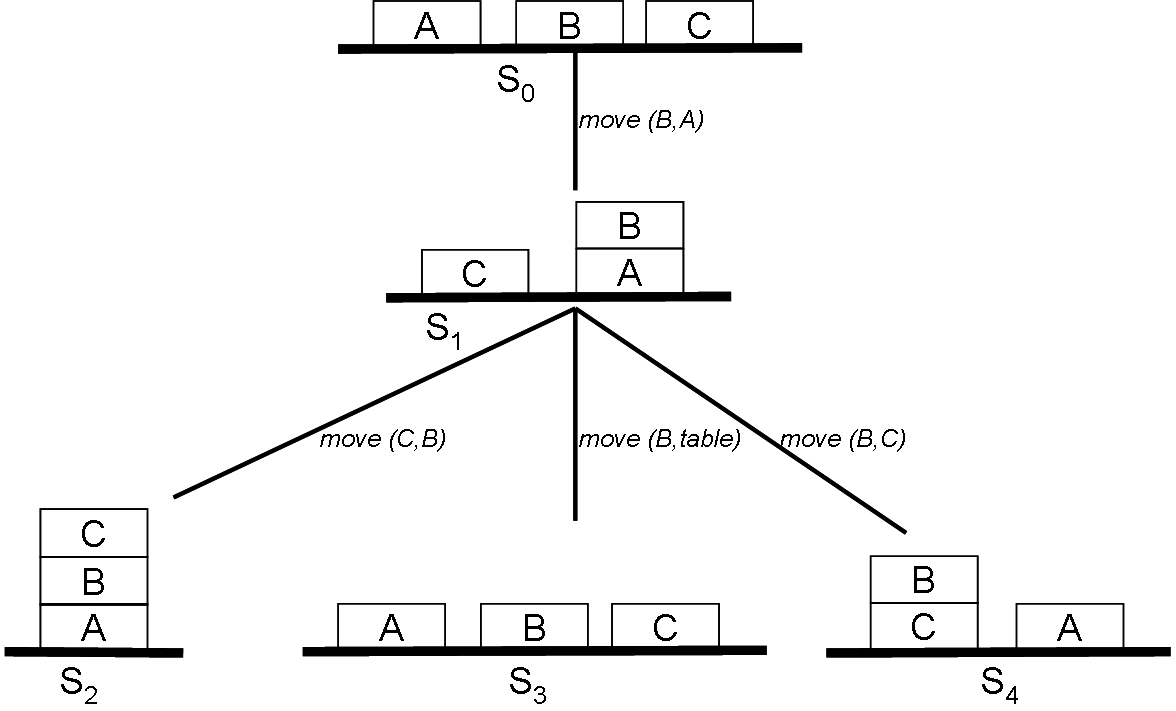
\includegraphics[scale=0.6]{3/eg1.png}
\caption{Example 1}
\label{fig:one}
\end{center}
\end{figure}
\begin{figure}[h]
\begin{center}
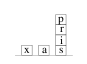
\includegraphics[scale=2]{3/eg2.png}
\caption{Example 2}
\label{fig:two}
\end{center}
\end{figure}

\section{\uppercase{View of Equations}}
The sum of squares of $a$ and $b$ are calculated as shown below:
\begin{eqnarray}
 \label{eq:sum}
 (a+b)^2 = a^2+b^2+2ab
\end{eqnarray}

From Equation \ref{eq:sum}, the data is obtained.





